\documentclass{cssheet}

%--------------------------------------------------------------------------------------------------------------
% Basic meta data
%--------------------------------------------------------------------------------------------------------------
\usepackage{tikz}
\usepackage{pgfplots}

\title{Kopfrechnen}
\author{Marvin Ködding \& Christian Spannagel}
\date{\today}
\hypersetup{%
    pdfauthor={\theauthor},%
    pdftitle={\thetitle},%
    pdfsubject={Aufgabenblatt Inside Math!},%
    pdfkeywords={insidemath}
}

%--------------------------------------------------------------------------------------------------------------
% document
%--------------------------------------------------------------------------------------------------------------

\begin{document}
\printtitle

\begin{aufgabe}[Funktionen finden]
	Findet funktionale Zusammenhänge in eurem Alltag. Untersucht diese unter dem Zuordnungsaspekt und Kovariationsaspekt.
\end{aufgabe}

\begin{aufgabe}[Füllgraphen]
	In die folgenden Gefäße wird mit einer konstanten \glqq{}Geschwindigkeit\grqq{} Wasser eingefüllt. Zeichnet einen Graphen, der die Füllhöhe des Wassers in Abhängigkeit der vergangenen Zeit darstellt.
	
	\begin{minipage}{.33\textwidth}
		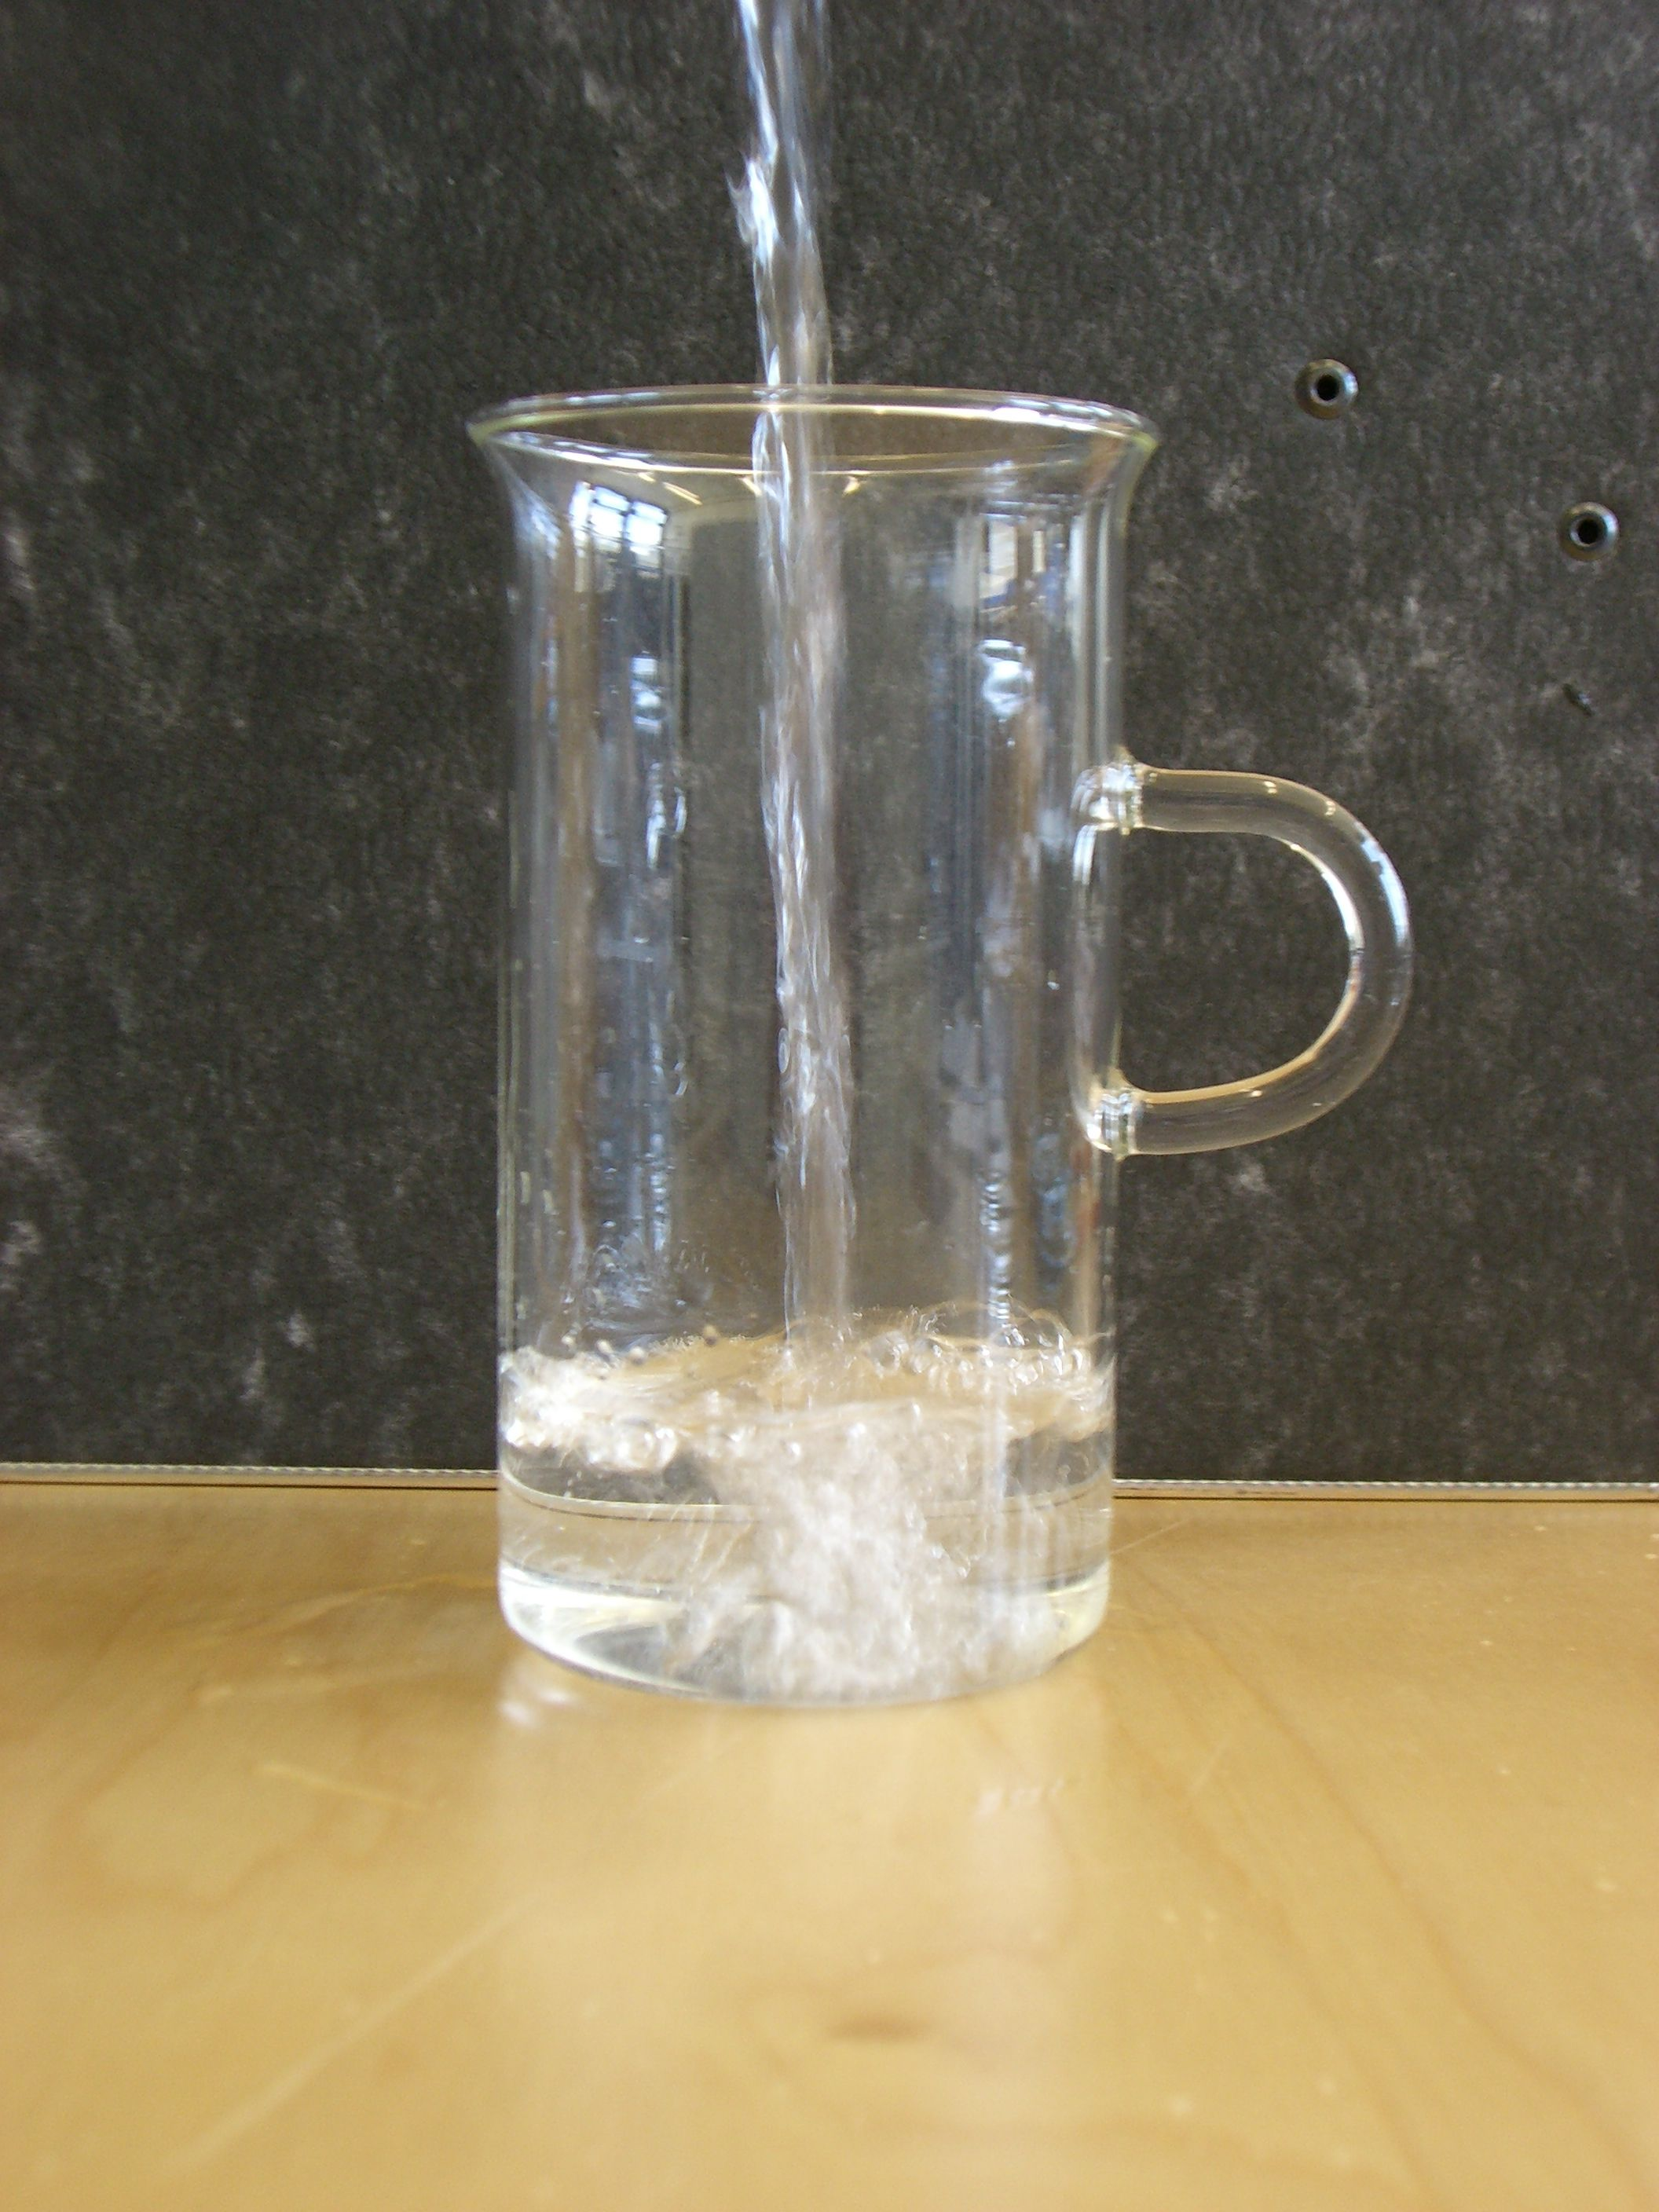
\includegraphics[width=\linewidth]{Gefaess_A_1.jpg}
	\end{minipage}
	\begin{minipage}{.33\textwidth}
		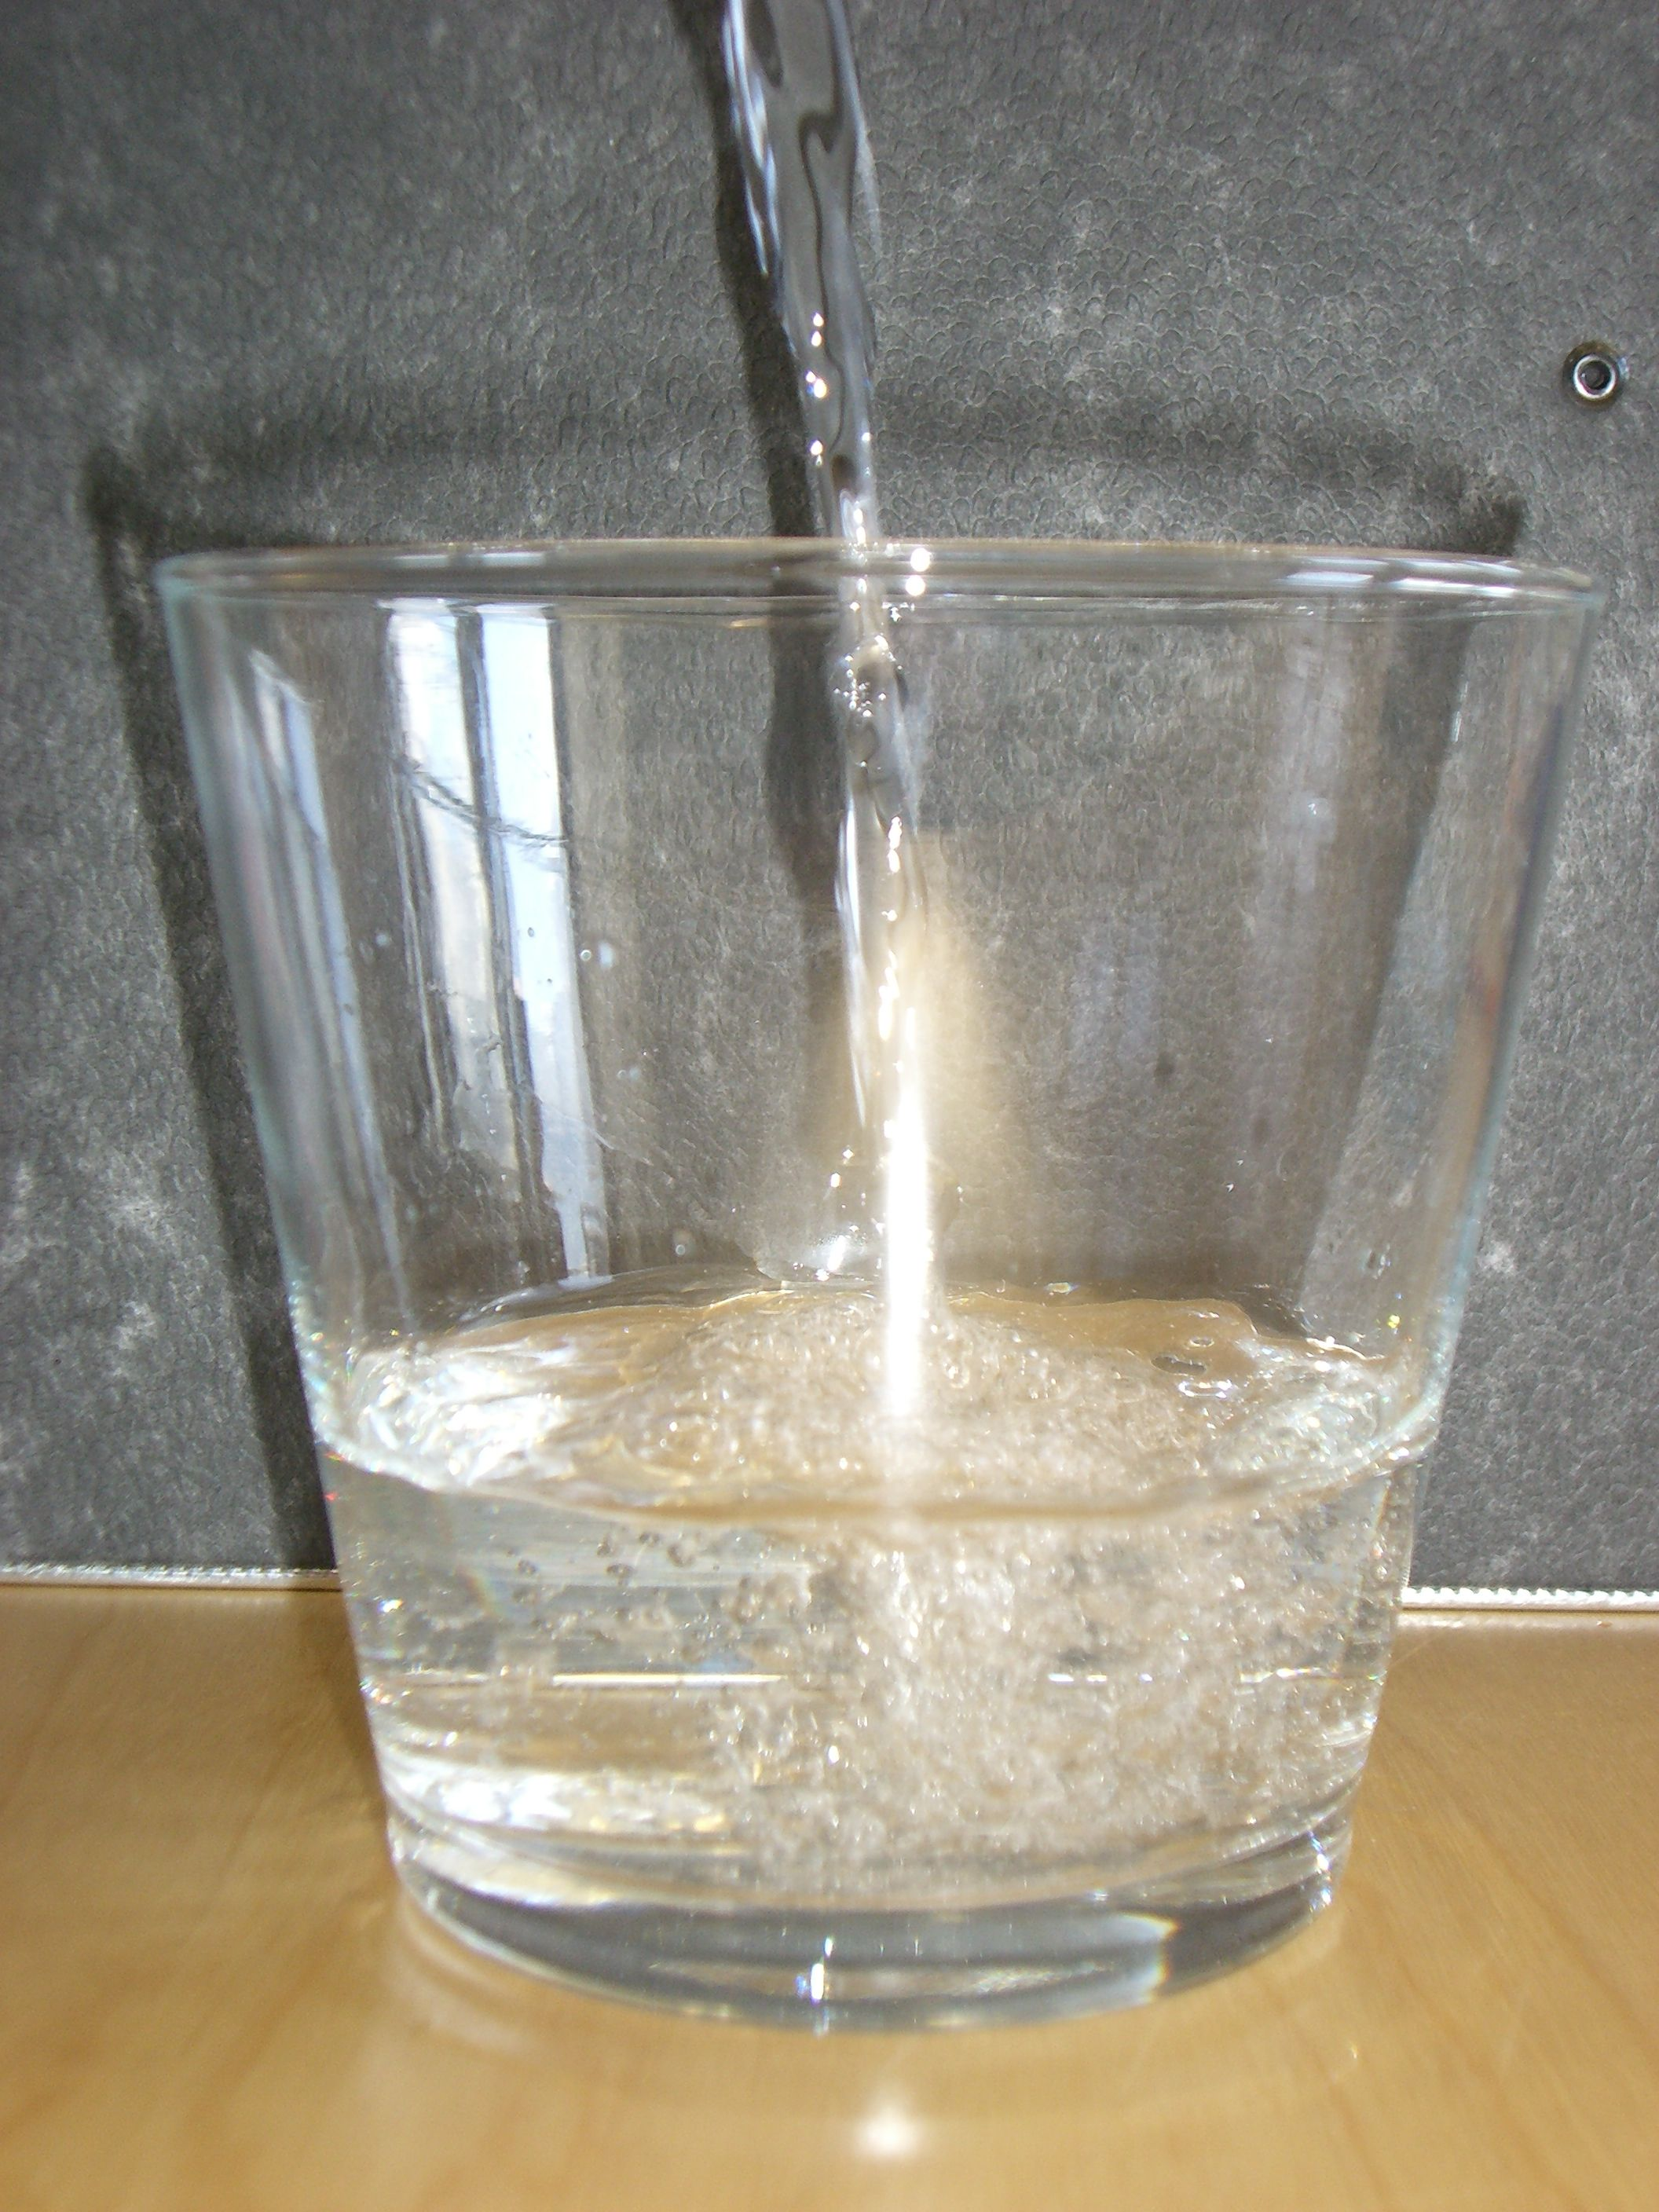
\includegraphics[width=\linewidth]{Gefaess_B_1.jpg}
	\end{minipage}
	\begin{minipage}{.33\textwidth}
		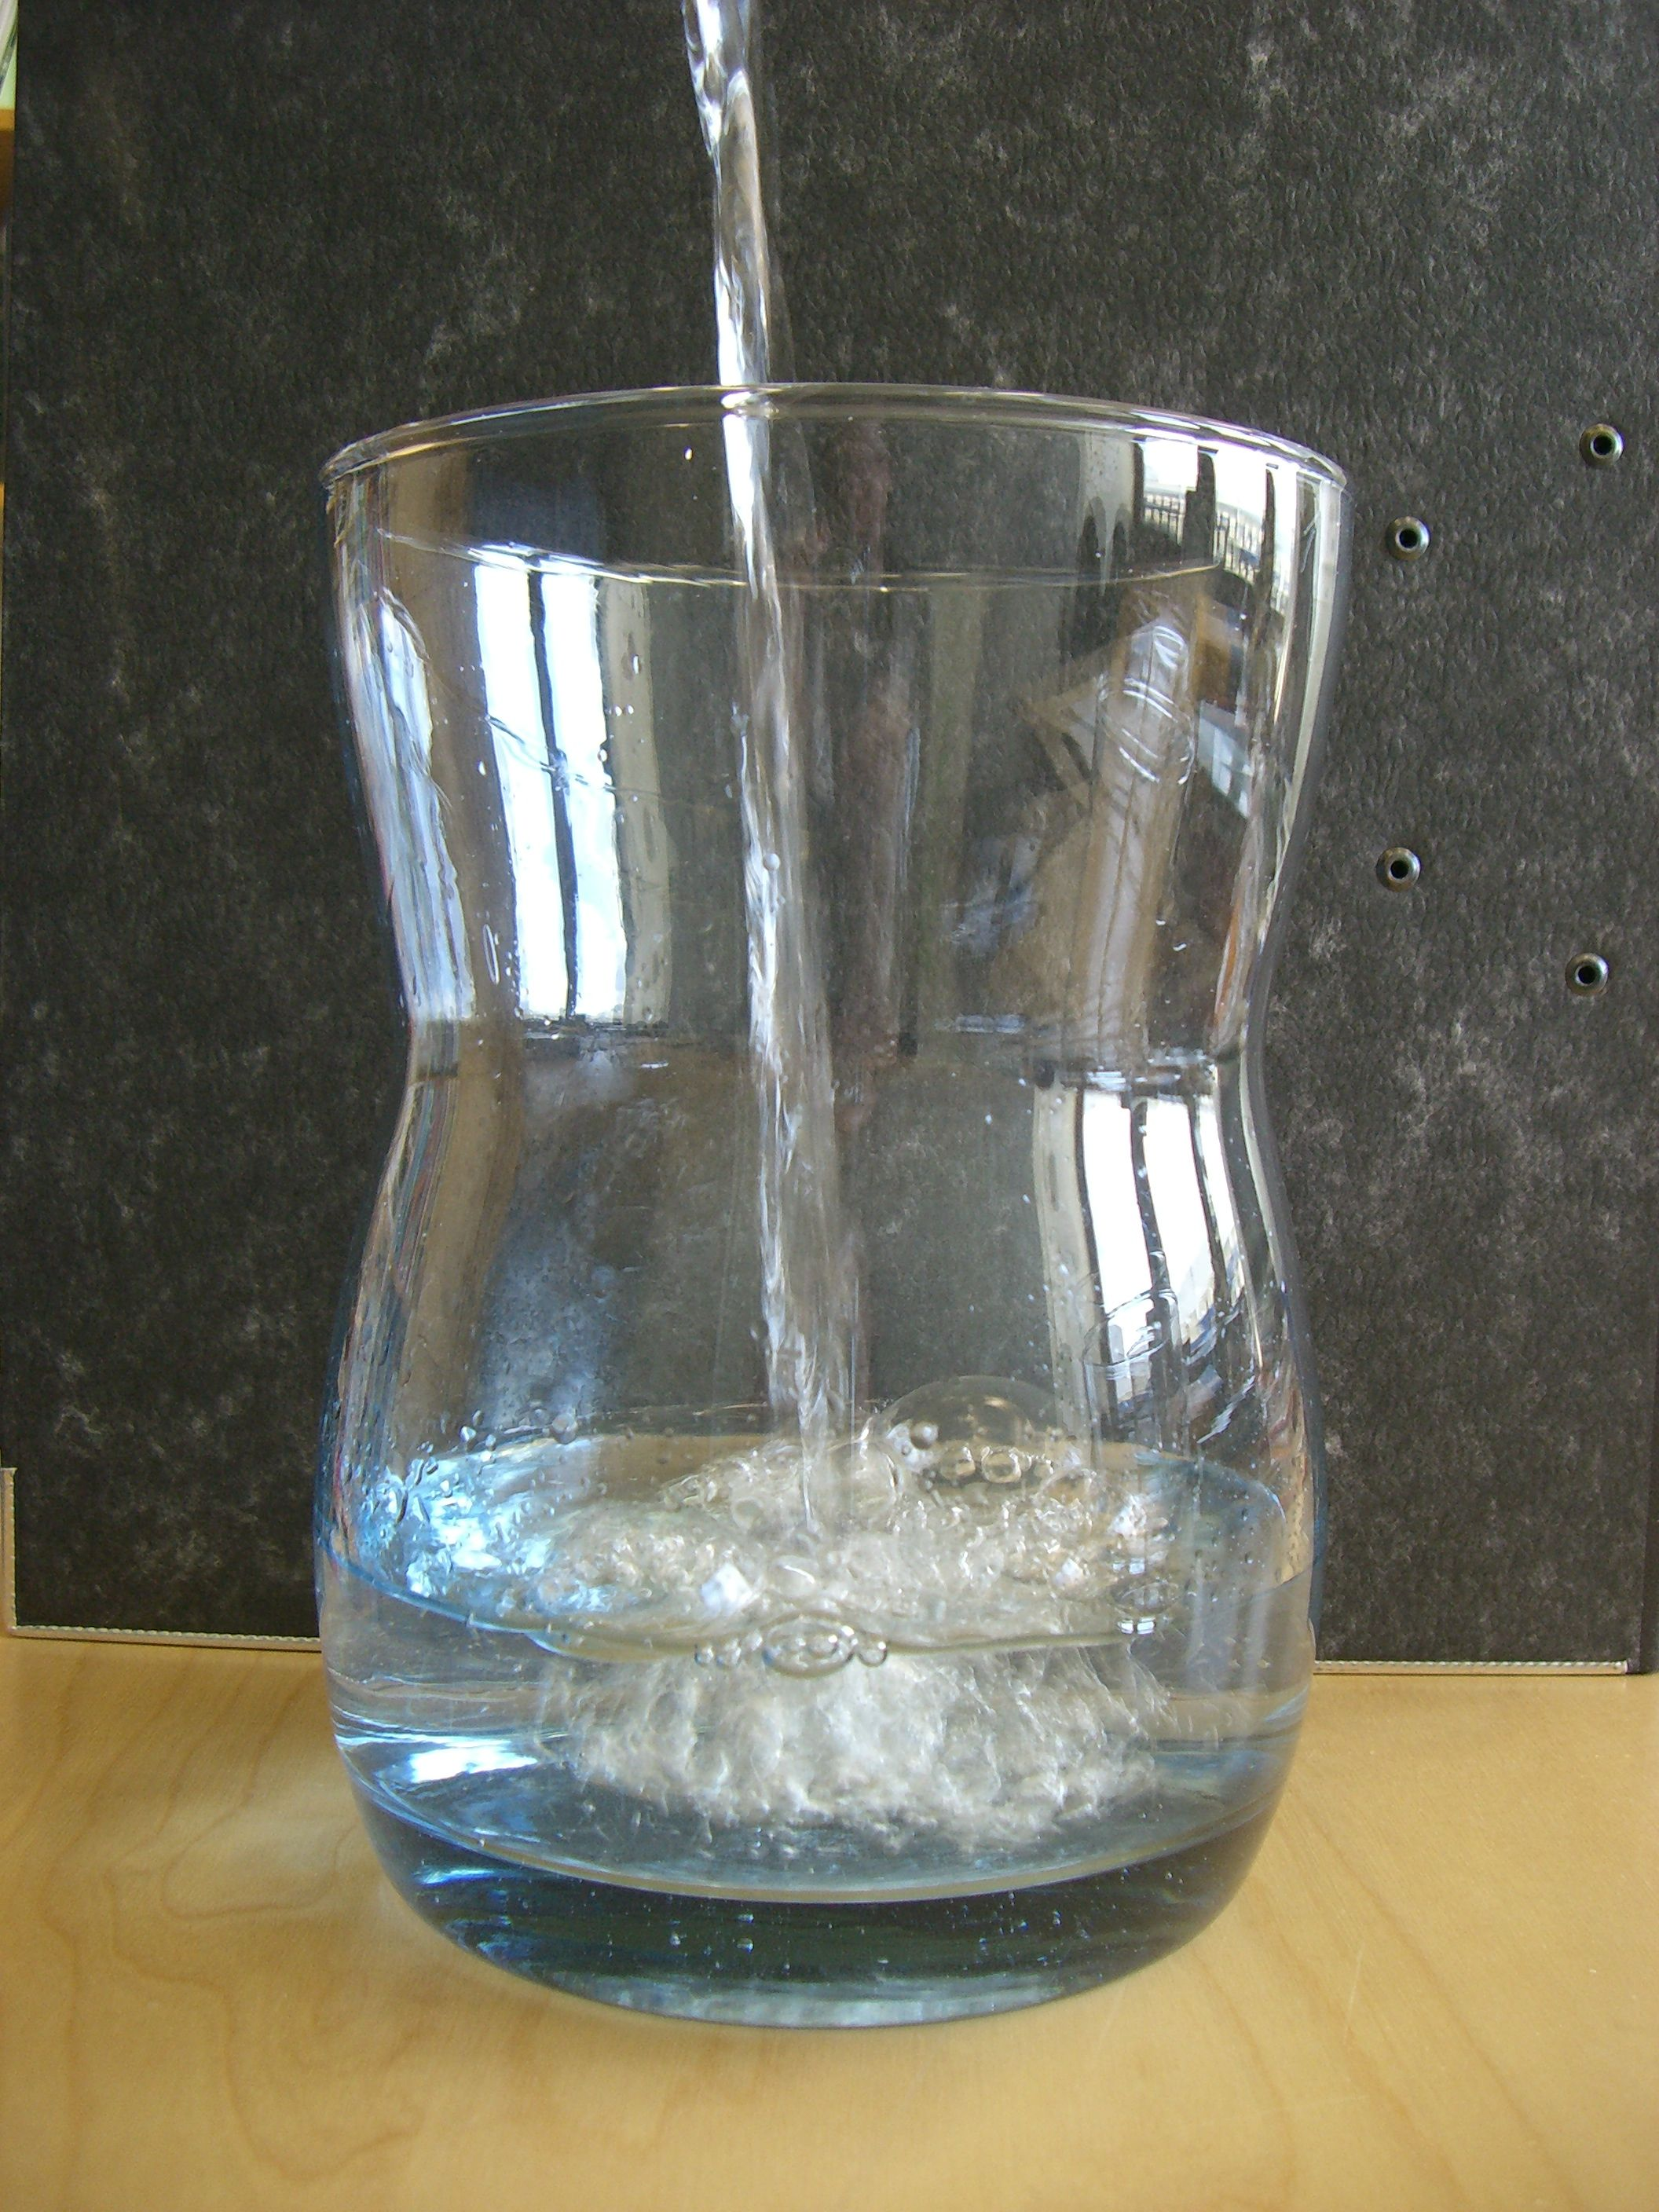
\includegraphics[width=\linewidth]{Gefaess_C_1.jpg}
	\end{minipage}
\end{aufgabe}

\begin{aufgabe}
	Zeichnet Gefäße, zu denen folgende Füllgraphen gehören könnten.
	
	\begin{center}
		\begin{minipage}{.4\textwidth}
			\scalebox{0.7}{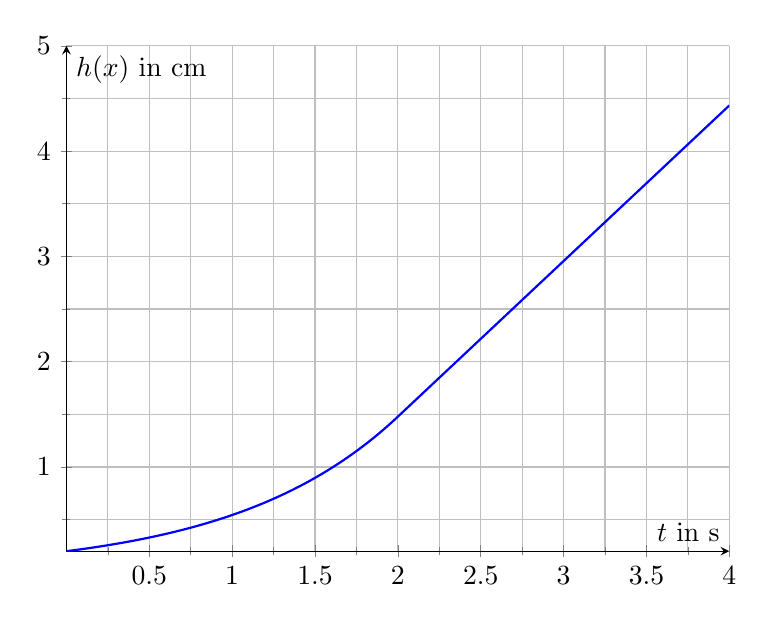
\begin{tikzpicture}
					\begin{axis}[
						axis lines = middle,
						xlabel = $t$ in s,
						ylabel = {$h(x)$ in cm},
						domain=0:4,
						samples=100,
						grid = both,
						minor tick num=1,
						width=10cm,
						height=8cm,
						ymax = 5
						]
						\addplot[
						thick,
						blue,
						domain=0:2
						]{0.2*exp(x)};
						\addplot[
						thick,
						blue,
						domain=2:4
						]{1.4778*x-1.4778};
					\end{axis}
			\end{tikzpicture}}
		\end{minipage}
		\begin{minipage}{.4\textwidth}
		\scalebox{0.7}{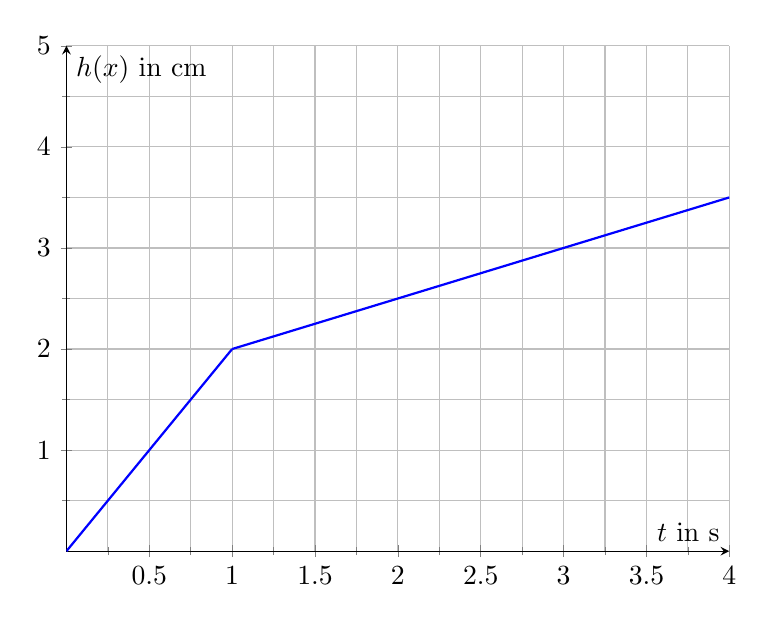
\begin{tikzpicture}
				\begin{axis}[
					axis lines = middle,
					xlabel = $t$ in s,
					ylabel = {$h(x)$ in cm},
					domain=0:4,
					samples=100,
					grid = both,
					minor tick num=1,
					width=10cm,
					height=8cm,
					ymax = 5
					]
					\addplot[
					thick,
					blue,
					domain=0:1
					]{2*x};
					\addplot[
					thick,
					blue,
					domain=1:4
					]{1/2 * x + 3/2};
				\end{axis}
		\end{tikzpicture}}
	\end{minipage}
	\end{center}
\end{aufgabe}

\newpage
\begin{aufgabe}[Zaubertruhe]
	In einer Zaubertruhe befindet sich eine Münze. Jede Minute verdoppelt sich die Anzahl der Münzen in der Zaubertruhe. Nach einer Stunde ist die Zaubertruhe voll. \begin{enumerate}
		\item Wann war die Zaubertruhe halb voll? \textit{Ihr könnt euch hier eine Wertetabelle mit Excel erstellen.}
		\item Findet einen Funktionsterm, der die Anzahl an Münzen in Abhängigkeit der vergangenen Minuten angibt.
		\item Um welchen Typ von Funktion handelt es sich?
	\end{enumerate}
\end{aufgabe}

\begin{aufgabe}[Hasengehege]
	Ein rechteckiges Hasengehege soll mit 20 m Zaun
	gebaut werden. Die Fläche des Hasengeheges soll möglichst
	groß sein. 
	\begin{enumerate}
		\item Welche Größen hängen hier voneinander ab? Stellt einen Funktionsterm auf.
		\item Welche Längen haben die Seiten des rechteckigen Hasengeheges mit der größten Fläche?
	\end{enumerate}
\end{aufgabe}

\vspace*{10mm}
\printlicense

\printsocials

\end{document}
